%%%%%%%%%%%%%%%%%%%%%%%%%%%%%%%%%%%%%%%%% 
% Beamer Presentation
% LaTeX Template
% Version 1.0 (10/11/12)
% 
% This template has been downloaded from:
% http://www.LaTeXTemplates.com
% 
% License:
% CC BY-NC-SA 3.0 (http://creativecommons.org/licenses/by-nc-sa/3.0/)
% 
%%%%%%%%%%%%%%%%%%%%%%%%%%%%%%%%%%%%%%%%% 

% ----------------------------------------------------------------------------------------
%	PACKAGES AND THEMES
% ----------------------------------------------------------------------------------------

\documentclass{beamer}

\mode<presentation> {

  % The Beamer class comes with a number of default slide themes
  % which change the colors and layouts of slides. Below this is a list
  % of all the themes, uncomment each in turn to see what they look like.

  % \usetheme{default}
  % \usetheme{AnnArbor}
  % \usetheme{Antibes}
  % \usetheme{Bergen}
  % \usetheme{Berkeley}
  % \usetheme{Berlin}
  % \usetheme{Boadilla}
  % \usetheme{CambridgeUS}
  % \usetheme{Copenhagen}
  % \usetheme{Darmstadt}
  % \usetheme{Dresden}
  % \usetheme{Frankfurt}
  % \usetheme{Goettingen}
  % \usetheme{Hannover}
  % \usetheme{Ilmenau}
  \usetheme{JuanLesPins}
  % \usetheme{Luebeck}
  % \usetheme{Madrid}
  % \usetheme{Malmoe}
  % \usetheme{Marburg}
  % \usetheme{Montpellier}
  % \usetheme{PaloAlto}
  % \usetheme{Pittsburgh}
  % \usetheme{Rochester}
  % \usetheme{Singapore}
  % \usetheme{Szeged}
  % \usetheme{Warsaw}

  % As well as themes, the Beamer class has a number of color themes
  % for any slide theme. Uncomment each of these in turn to see how it
  % changes the colors of your current slide theme.

  % \usecolortheme{albatross}
  % \usecolortheme{beaver}
  % \usecolortheme{beetle}
  % \usecolortheme{crane}
  % \usecolortheme{dolphin}
  % \usecolortheme{dove}
  % \usecolortheme{fly}
  % \usecolortheme{lily}
  % \usecolortheme{orchid}
  % \usecolortheme{rose}
  % \usecolortheme{seagull}
  % \usecolortheme{seahorse}
  % \usecolortheme{whale}
  % \usecolortheme{wolverine}

  % \setbeamertemplate{footline} % To remove the footer line in all slides uncomment this line
  % \setbeamertemplate{footline}[page number] % To replace the footer line in all slides with a simple slide count uncomment this line

  % \setbeamertemplate{navigation symbols}{} % To remove the navigation symbols from the bottom of all slides uncomment this line
}

\usepackage{graphicx} % Allows including images
\usepackage{multirow}
\usepackage{booktabs} % Allows the use of \toprule, \midrule and \bottomrule in tables
\graphicspath{ {images/} }

% ----------------------------------------------------------------------------------------
%	TITLE PAGE
% ----------------------------------------------------------------------------------------

\title[Web Development Backend Introduction]{Web BE Introduction} % The short title appears at the bottom of every slide, the full title is only on the title page

\author{Guanyu Yi} % Your name
\institute[Alchip] % Your institution as it will appear on the bottom of every slide, may be shorthand to save space
{
  OP Team, Alchip, Inc. \\ % Your institution for the title page
  \medskip
  \textit{guanyu\_yi@alchip.com} % Your email address
}
\date{July 6, 2018} % Date, can be changed to a custom date

\AtBeginSection
{
  \begin{frame}
    \tableofcontents[currentsection]
  \end{frame}
}

\begin{document}

\begin{frame}
  \titlepage % Print the title page as the first slide
\end{frame}

\begin{frame}
  \frametitle{Overview} % Table of contents slide, comment this block out to remove it
  \tableofcontents[subsectionstyle=hide] % Throughout your presentation, if you choose to use \section{} and \subsection{} commands, these will automatically be printed on this slide as an overview of your presentation
\end{frame}

% ----------------------------------------------------------------------------------------
%	PRESENTATION SLIDES
% ----------------------------------------------------------------------------------------

% ------------------------------------------------
\section{Database} % Sections can be created in order to organize your presentation into discrete blocks, all sections and subsections are automatically printed in the table of contents as an overview of the talk

\subsection{Concept}

\begin{frame}
  \begin{columns}[c] % The "c" option specifies centered vertical alignment while the "t" option is used for top vertical alignment

    \column{.45\textwidth} % Left column and width
    \begin{figure}
      \centering
      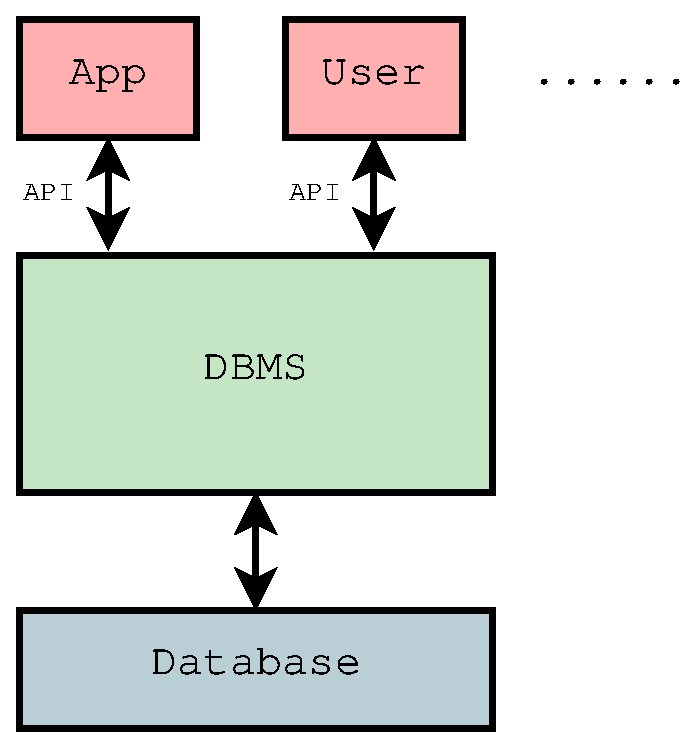
\includegraphics[width=0.65\linewidth]{dbms}
      \caption{DBMS Architecture}
    \end{figure}

    \column{.45\textwidth} % Left column and width
    \begin{figure}
      \centering
      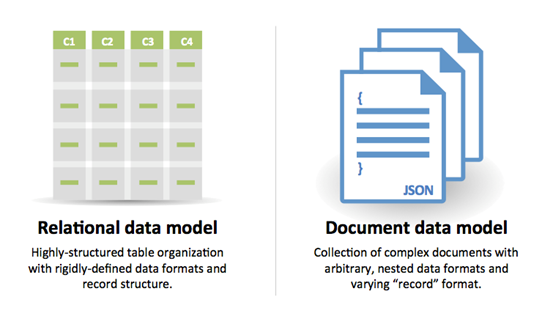
\includegraphics[width=1.25\linewidth]{sql_vs_nosql}
      \caption{SQL vs NoSQL}
    \end{figure}
    
  \end{columns}
\end{frame}

% ----------------------------------------------------------------------------------------

% ------------------------------------------------
\subsection{Schema \& Data} % Sections can be created in order to organize your presentation into discrete blocks, all sections and subsections are automatically printed in the table of contents as an overview of the talk

\begin{frame}
  \begin{figure}
    \centering
    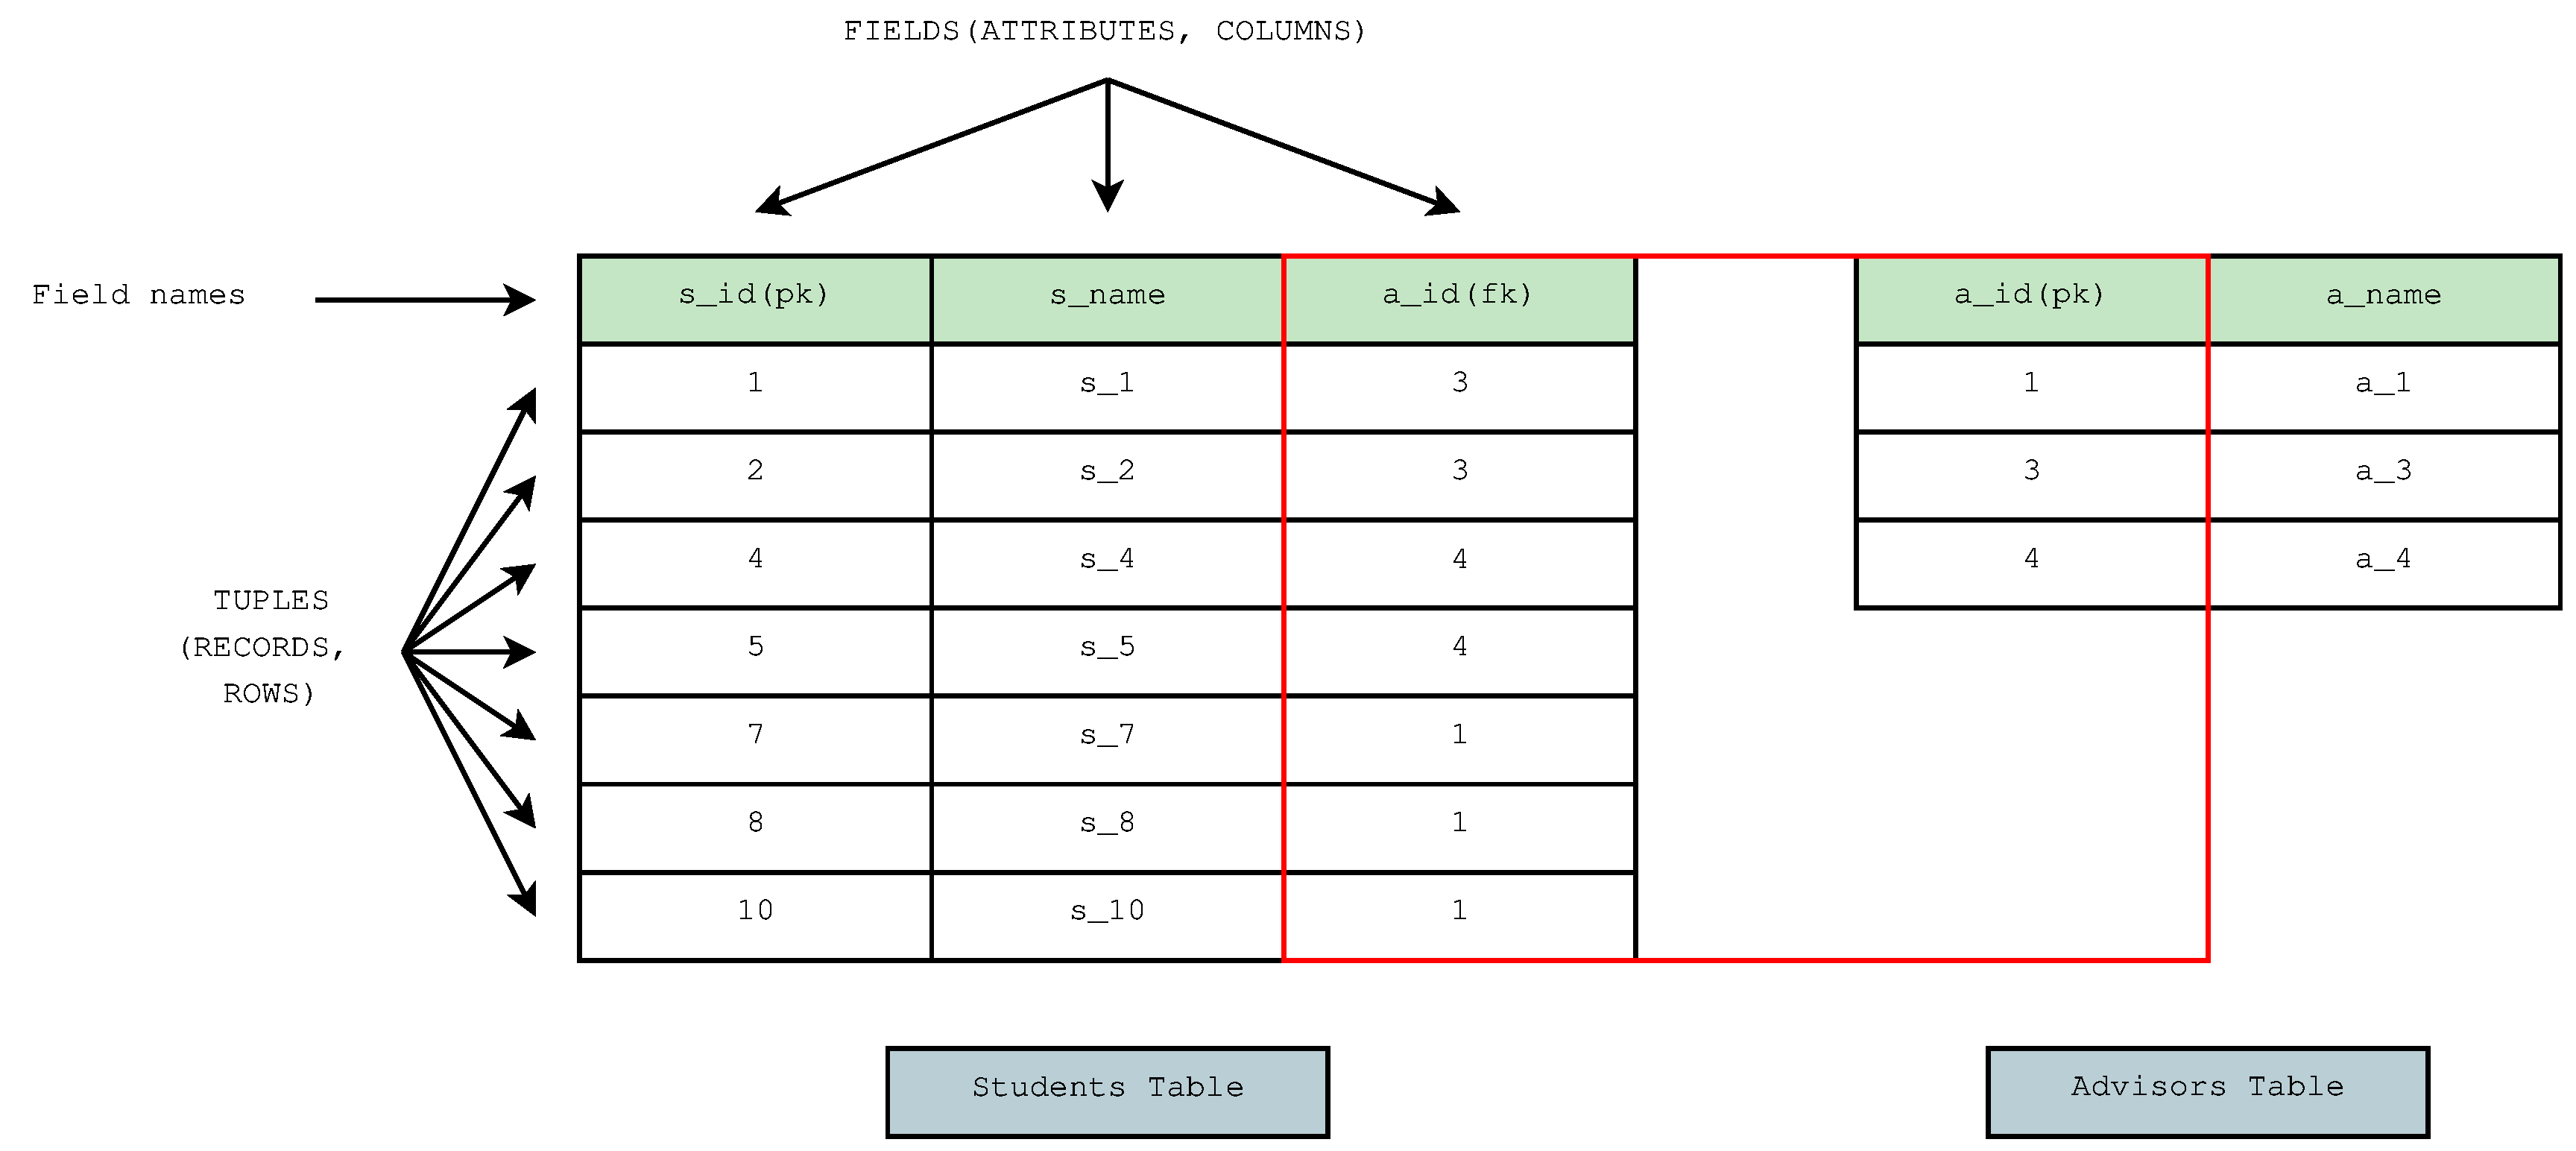
\includegraphics[width=1.05\linewidth]{schema}
    \caption{Example Tables}
  \end{figure}
\end{frame}
% ----------------------------------------------------------------------------------------

% ------------------------------------------------
\subsection{SQL} % Sections can be created in order to organize your presentation into discrete blocks, all sections and subsections are automatically printed in the table of contents as an overview of the talk

\begin{frame}
  \begin{figure}
    \centering
    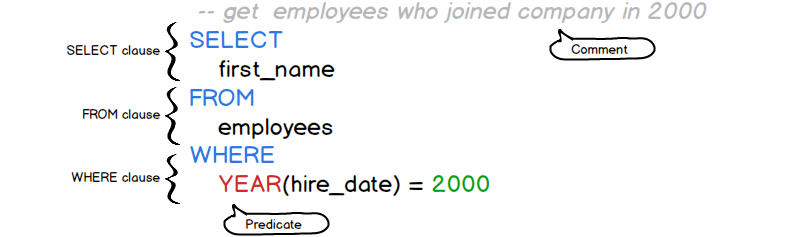
\includegraphics[width=1.05\linewidth]{sql_syntax}
    \caption{SQL}
  \end{figure}
\end{frame}
% ----------------------------------------------------------------------------------------

% ------------------------------------------------
\section{ORM} % Sections can be created in order to organize your presentation into discrete blocks, all sections and subsections are automatically printed in the table of contents as an overview of the talk

\subsection{Concept}

\begin{frame}
  \begin{figure}
    \centering
    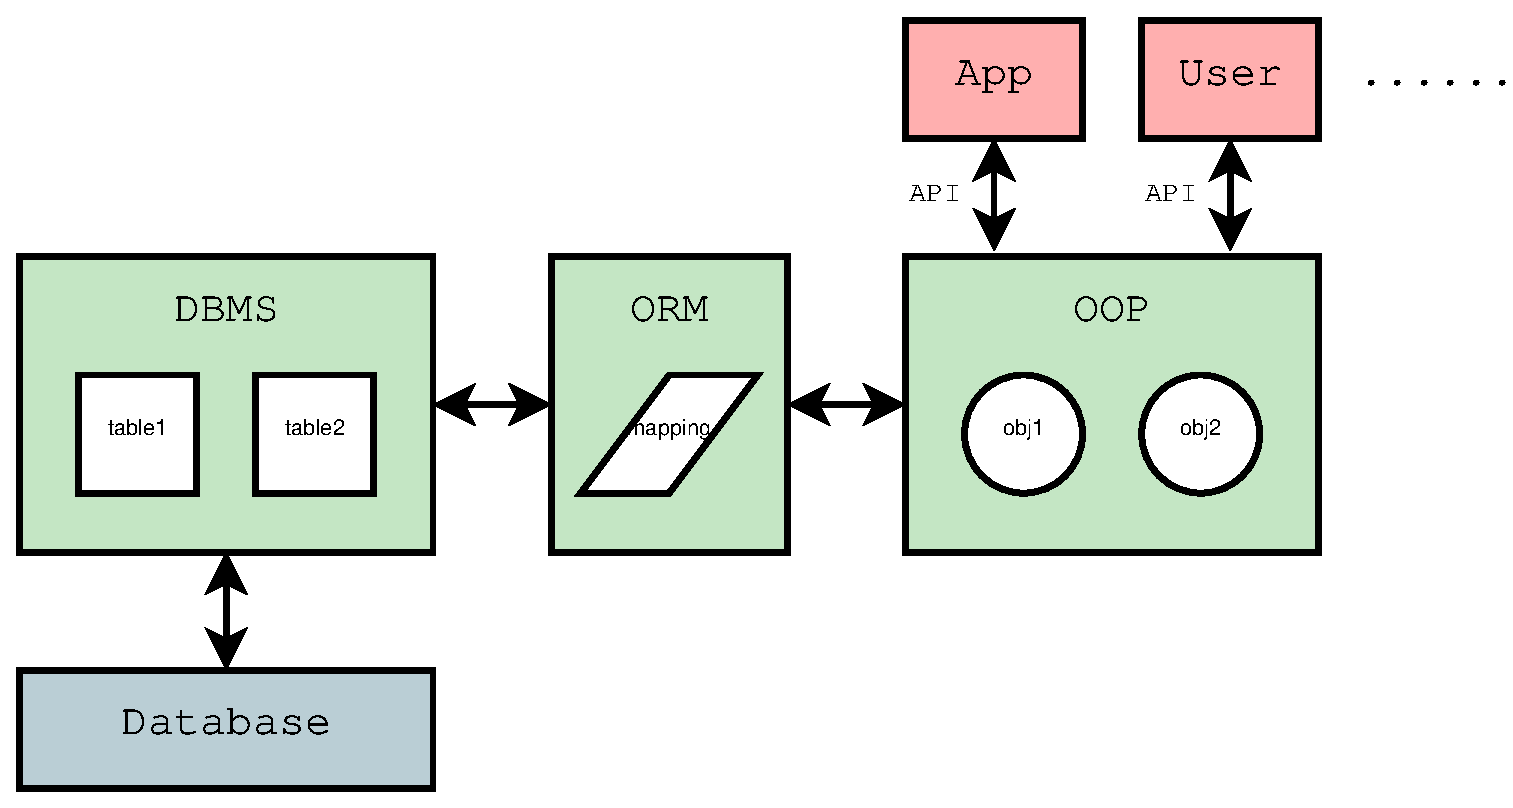
\includegraphics[width=1.05\linewidth]{orm}
    \caption{Object Relational Mapping}
  \end{figure}
\end{frame}
% ----------------------------------------------------------------------------------------

% ------------------------------------------------
\subsection{ORM vs SQL} % Sections can be created in order to organize your presentation into discrete blocks, all sections and subsections are automatically printed in the table of contents as an overview of the talk

\begin{frame}
  \begin{figure}
    \centering
    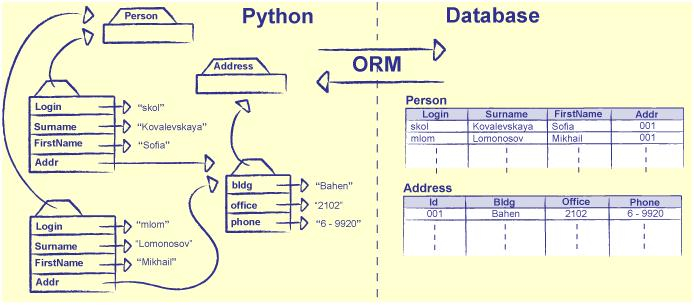
\includegraphics[width=1.05\linewidth]{orm_vs_sql}
    \caption{ORM vs SQL}
  \end{figure}
\end{frame}
% ----------------------------------------------------------------------------------------

% ------------------------------------------------
\section{Django} % Sections can be created in order to organize your presentation into discrete blocks, all sections and subsections are automatically printed in the table of contents as an overview of the talk

\subsection{Architecture}
\begin{frame}
  \begin{columns}[c] % The "c" option specifies centered vertical alignment while the "t" option is used for top vertical alignment

    \column{.45\textwidth} % Left column and width
    \begin{figure}
      \centering
      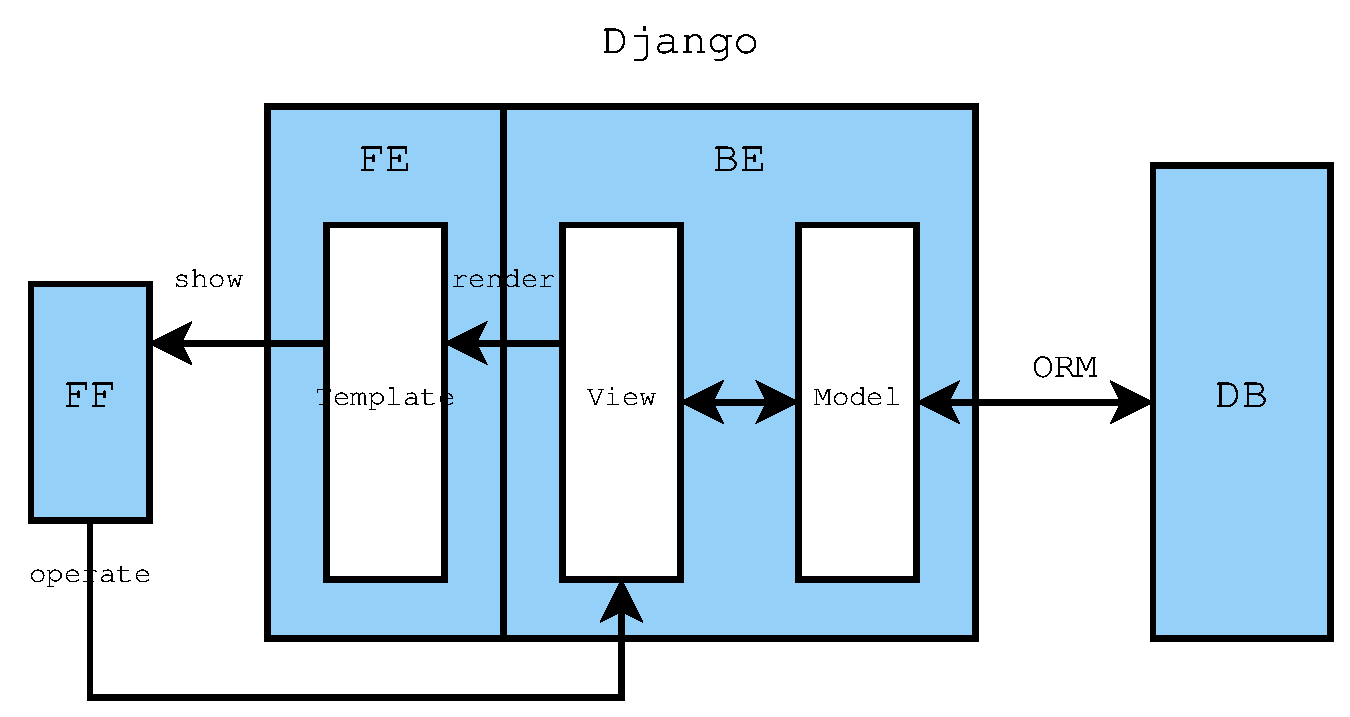
\includegraphics[width=1.10\linewidth]{django_arch}
      \caption{Django Architecture}
    \end{figure}

    \column{.45\textwidth} % Left column and width
    \begin{figure}
      \centering
      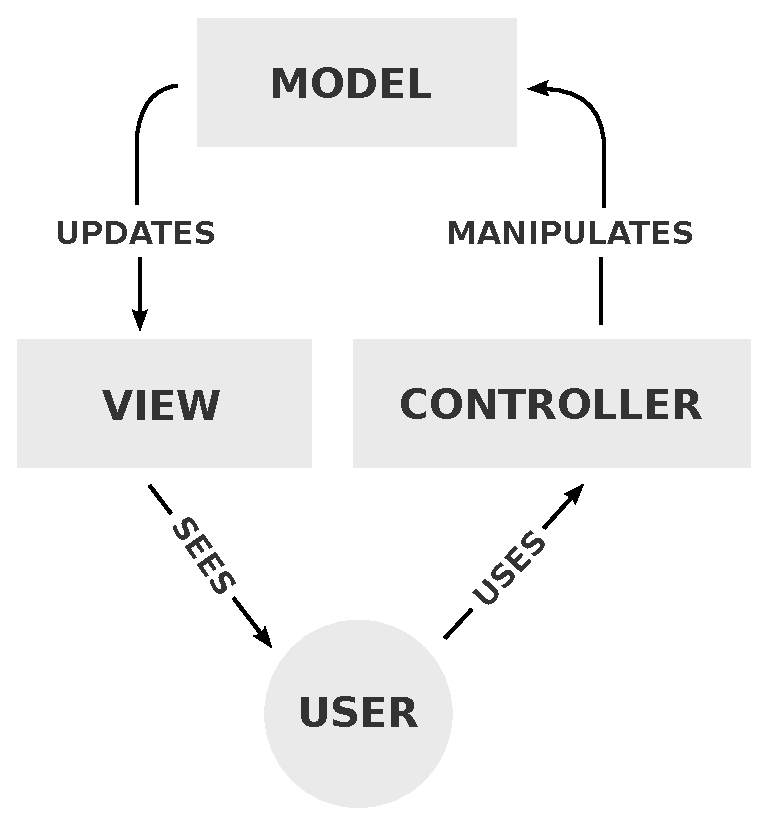
\includegraphics[width=0.90\linewidth]{mvc_process}
      \caption{MVC Architecture}
    \end{figure}

  \end{columns}
\end{frame}
% ----------------------------------------------------------------------------------------

% ------------------------------------------------
\subsection{Evolution} % Sections can be created in order to organize your presentation into discrete blocks, all sections and subsections are automatically printed in the table of contents as an overview of the talk

\begin{frame}
  \begin{figure}
    \centering
    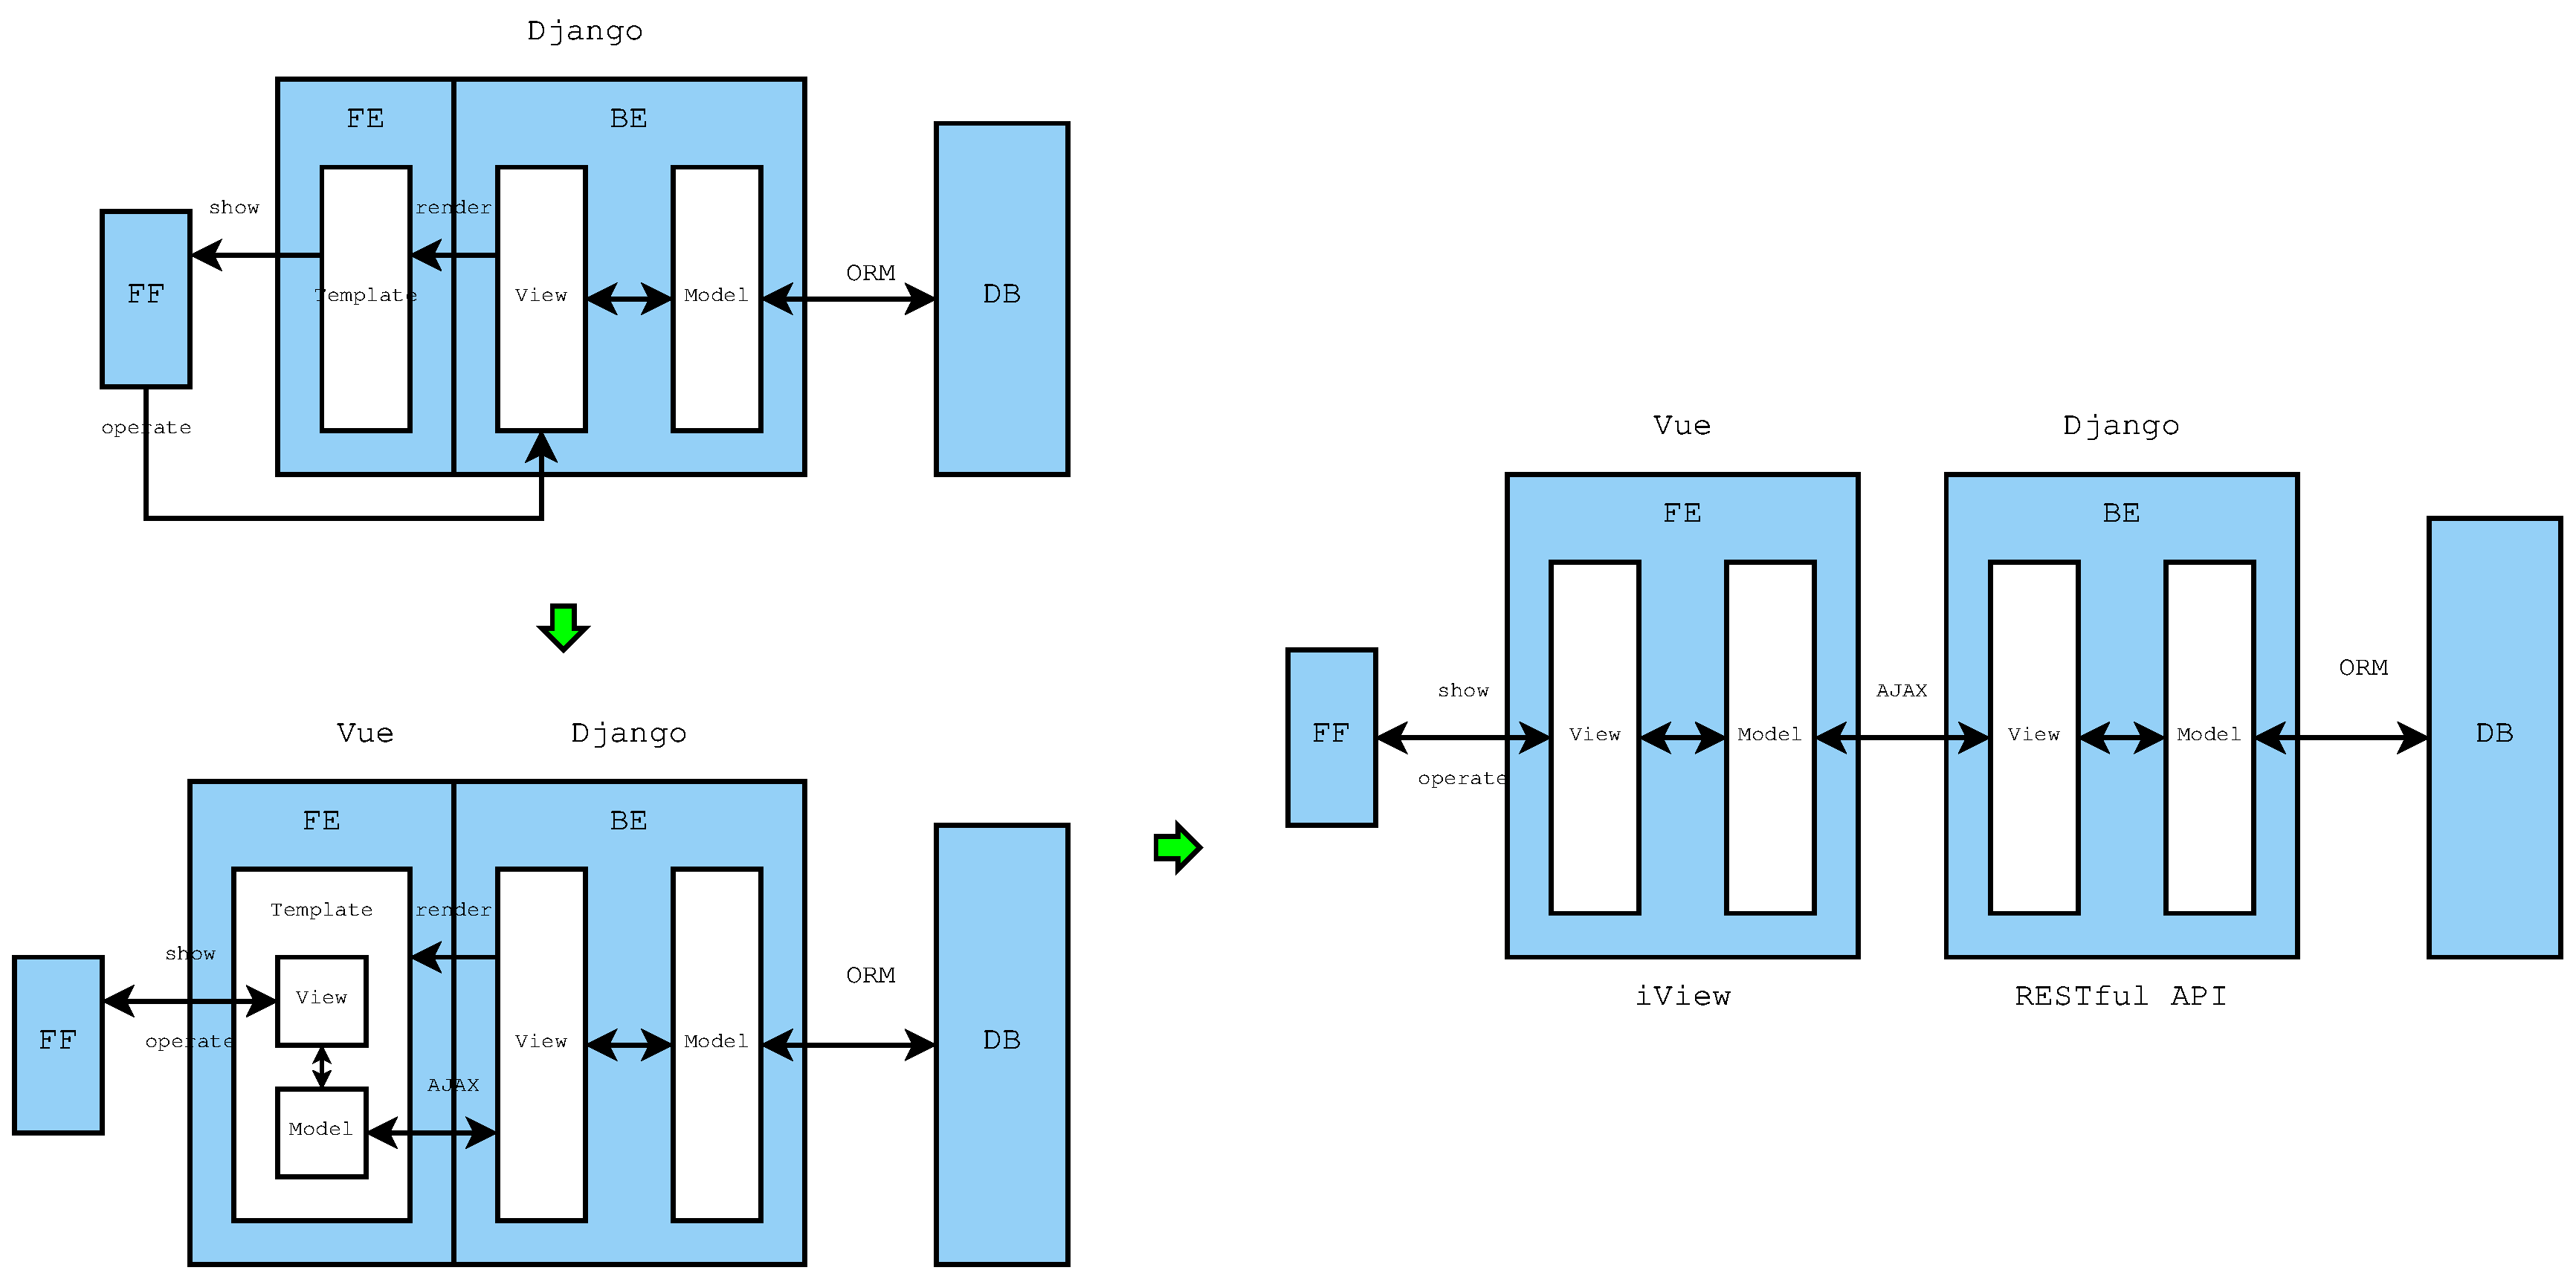
\includegraphics[width=1.05\linewidth]{web_evo}
    \caption{Web Development Evolution}
  \end{figure}
\end{frame}
% ----------------------------------------------------------------------------------------

% ----------------------------------------------------------------------------------------

\section{Q \& A}
\begin{frame}
  \Huge{\centerline{Q \& A}}
\end{frame}

% ----------------------------------------------------------------------------------------

\end{document} 
%%% Local Variables:
%%% mode: latex
%%% TeX-master: t
%%% End:
